\documentclass[a4paper]{article}

\usepackage[english]{babel}
\usepackage[utf8x]{inputenc}
\usepackage{amsmath}
\usepackage{graphicx}
\usepackage[colorinlistoftodos]{todonotes}

\title{CS 5785 -- Applied Machine Learning -- Lec.\ 6}
\author{Prof.\ Nathan Kallus, Cornell Tech\\Scribe: TBD}
\date{Sept.\ 7, 2017}

\begin{document}
\maketitle


\section{Multivariate Gaussian/Normal Density}
One of the most commonly used pdfs in engineering is the multivariate Gaussian or normal density:
\begin{equation}
f_k(x)=\frac{1}{(2\pi)^{p/2}|\Sigma_k|^{1/2}}e^{-\frac{1}{2}(x-\mu_k)^\top\Sigma_k^{-1}(x-\mu_k)}
\label{eqn:mvgaussian}
\end{equation}
 The constant term $\frac{1}{(2\pi)^{p/2}|\Sigma_k|^{1/2}}$ ensures that $f_k(x)$ integrates to 1.  For additional intuition, plug in $p=1$  and see that it reduces to the familiar \emph{univariate} (or 1D) Gaussian density, parameterized by a mean $\mu$ and variance $\sigma^2$.  The equation (1) will come down to:
\begin{equation}
f(x) = \frac{1}{\sqrt{2\pi\sigma^2}}e^{-\frac{(x-\mu)^2}{2\sigma^2}}
\end{equation}

In particular, we often use multivariate normals as \emph{class conditional densities}, e.g., to describe the height and weight of a pet given that it is a dog.  We say ``$X$ conditioned on class $k$ is normally distributed'' and write:
\begin{equation}
X|G=k\sim{\mathcal N}(\mu_k,\Sigma_k)
\end{equation}
In this expression, $\mu_k$ and $\Sigma_k$ represent the \emph{mean vector} and \emph{covariance matrix} of the density for the $k$th class, respectively, and $p$ is the number of dimensions of the feature vector $x$, as usual. The covariance matrix is sometimes called the variance-covariance matrix since the variances of the individual variables are on the diagonal and covariances are off-diagonal.

Figures \ref{fig:gaussian_contours} and \ref{fig:gaussian_heatmap} show two ways of visualizing this distribution for $p=2$, a special case known as a \emph{bivariate normal}.  Figure \ref{fig:gaussian_contours} highlights that the fact that the level sets of a bivariate Gaussian are ellipses.  Figure \ref{fig:gaussian_heatmap} shows three examples of bivariate Gaussians as surface plots and \emph{heatmaps}.  If the covariance matrix is represented by an identity matrix, the contour plots of probability density will be concentric circles. In any other case, looking at covariance matrices doesn't make  any sense, you can't predict it based on the values. Eigenvalues and eigenvectors should be used instead.

\begin{figure}
\centering
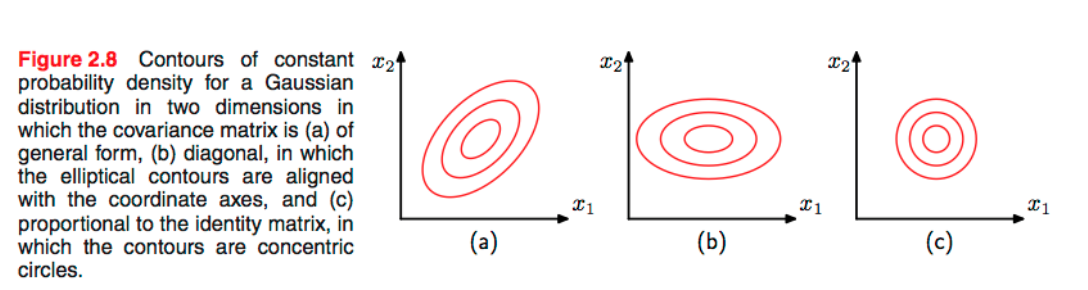
\includegraphics[width=1.0\textwidth]{gaussian_contours.png}
\caption{\label{fig:gaussian_contours}[Bishop]}
\end{figure}

\begin{figure}
\centering
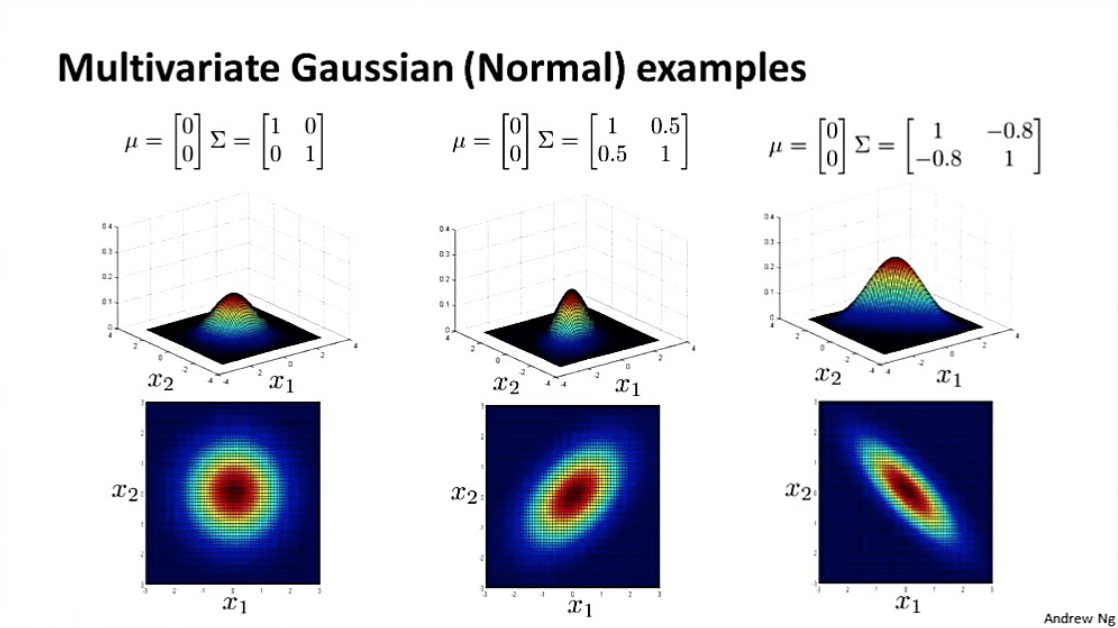
\includegraphics[width=1.0\textwidth]{gaussian_heatmap.png}
\caption{\label{fig:gaussian_heatmap}[A.\ Ng]}
\end{figure}


Figure \ref{fig:birdspace} shows an example of bivariate Gaussians used to model features of two birds (sandpiper vs.\ hawk).  In this example, we have two class conditional densities with different means but equal covariance matrices, and the features capture characteristics of the beak and color of the plumage.  The figure also foreshadows how we can use these densities to define a decision boundary.

\begin{figure}
\centering
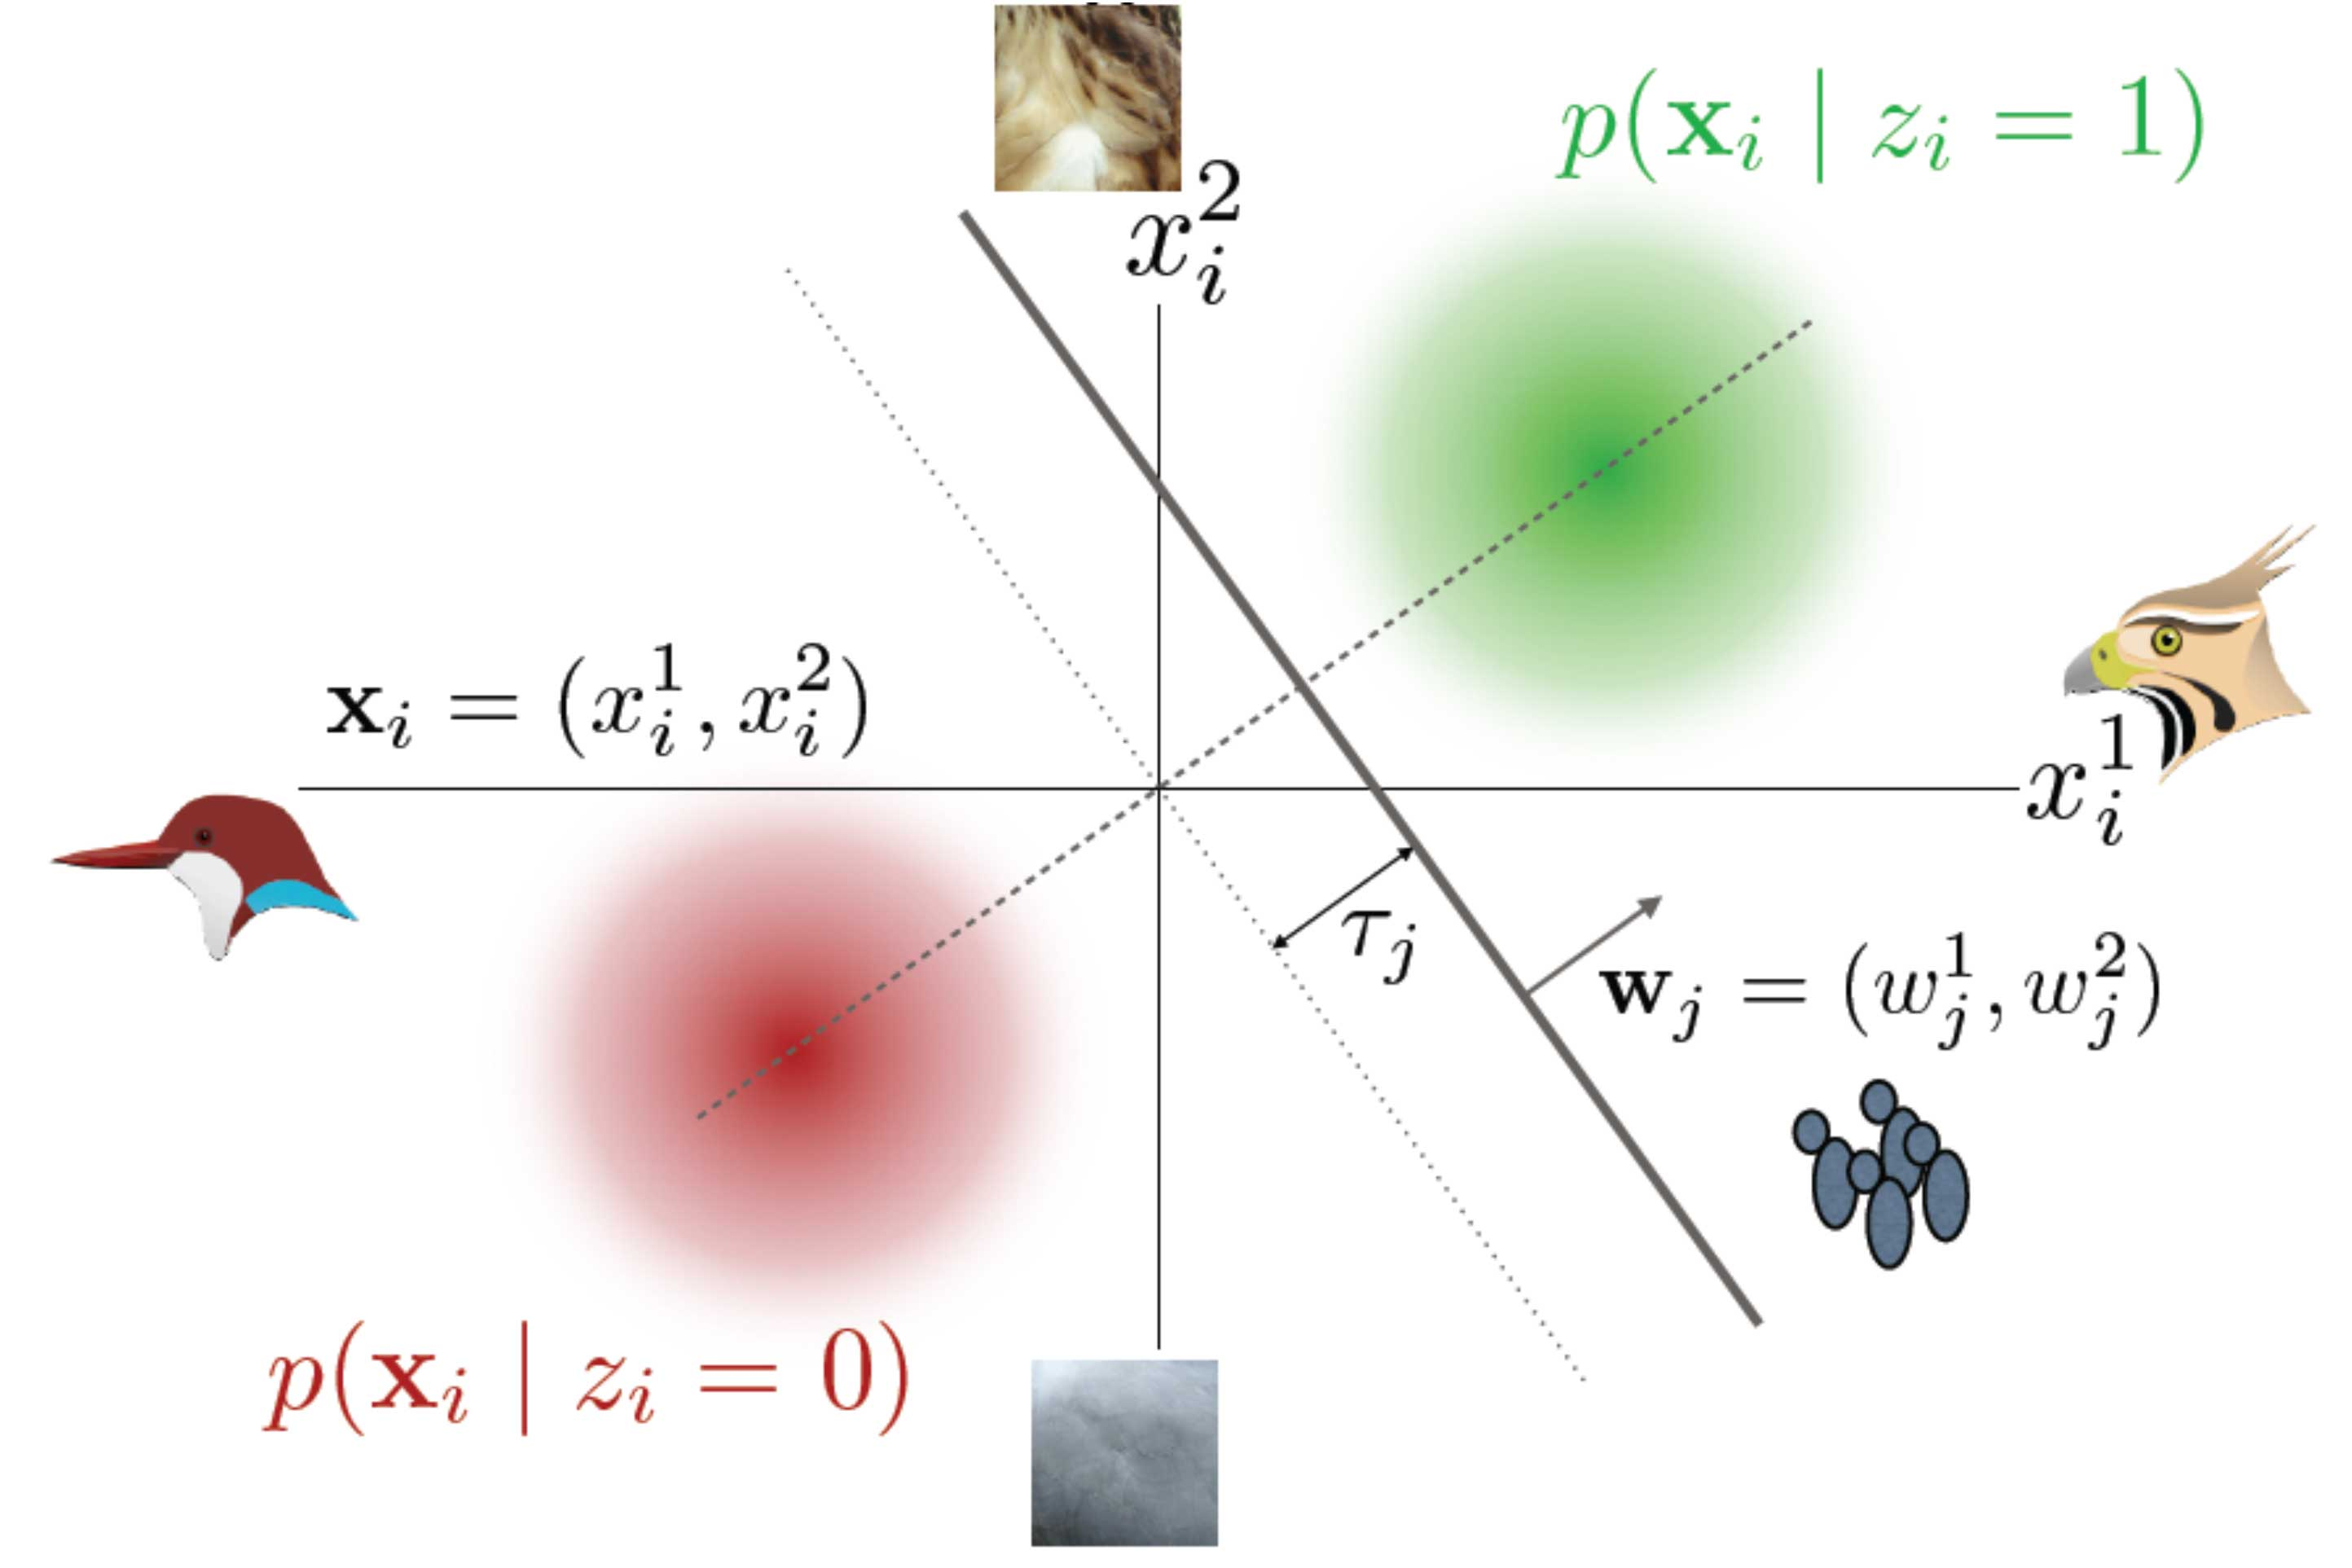
\includegraphics[width=0.75\textwidth]{welinder2010.jpg}
\caption{\label{fig:birdspace}[Welinder]}
\end{figure}


One practical limitation of the Gaussian is that it is \emph{unimodal}, which is another way of saying that the density just has one bump.  Such a density isn't a good fit for classes comprising distinct subclasses, e.g., the color of bell peppers.   Multimodal densities such as a \emph{Gaussian Mixture Models}, which we'll discuss later in the class, can address this problem.


\subsection{Quadratic Forms}
Look at the exponent in Equation \ref{eqn:mvgaussian}.  Assuming $\mu_k = 0$, which we refer to as the \emph{mean zero} or \emph{centered} case, $(x-\mu_k)^\top\Sigma_k^{-1}(x-\mu_k)$ has the form $f(x)=x^\top Qx$, which is known in linear algebra as a \emph{quadratic form}.  Looking at the dimensions of these terms, the exponent resolves to a scalar.  The entries in the matrix $Q$ control the shape of the function $f(x)$, as illustrated in Figure \ref{fig:gaussian_contours}.  An ellipse in that figure represents the locus of values $x$ such that $f(x)=x^\top Q x=\text{some constant}$.  In the case of Equation \ref{eqn:mvgaussian}, the covariance matrix $\Sigma_k^{-1}$ is \emph{positive definite}, a property that we will discuss later.  People often think of covariance matrices as ellipses: perfect circles mean no correlation.

This quadratic form is of interest to us since we often work with log likelihoods instead of raw likelihoods.  Returning to Equation \ref{eqn:mvgaussian}, when you take its log, you get the quadratic form discussed above.

\section{Linear Discriminant Analysis}
Linear Discriminant Analysis (LDA) is a supervised classification method that assumes the class conditional densities are Gaussian and that all of the covariance matrices are equal, i.e., $\Sigma_k=\Sigma$.  It can also be used for dimensionality reduction, which takes in very large feature vectors and collapses them into a small number of meaningful dimensions.  To see how it works, let $\pi_k$ denote the prior probability of class $k$ (which means $\sum_{k=1}^K \pi_k=1$) and apply Bayes' theorem to express the posterior probability as follows:
$$
Pr(G=k|X=x) = \frac{f_k(x)\pi_k}{\sum_{l=1}^K f_l(x)\pi_l}
$$
Recall that $f_k(x)$ is the class-conditional density and the denominator is the normalization factor or marginal likelihood.  Bayes' rule allows us to take the class conditional density and turn it around so we can predict the class given our data.
Assume for now that $\pi_k, \mu_k$ and $\Sigma_k$ are all known.  Now look at the log-odds we get by comparing two classes $k$ and $l$:
$$
\log \frac{Pr(G=k|X=x)}{Pr(G=l|X=x)}=\log\frac{f_k(x)}{f_l(x)}+\log\frac{\pi_k}{\pi_l}
$$
Notice how the log-odds on the priors appears as a constant offset or shift.
Assuming Gaussian class conditional densities, we get
$$
\log \frac{Pr(G=k|X=x)}{Pr(G=l|X=x)}=\log\frac{\pi_k}{\pi_l}-\frac{1}{2}(\mu_k+\mu_l)^\top\Sigma^{-1}(\mu_k-\mu_l)+x^\top\Sigma^{-1}(\mu_k-\mu_l)
$$
Note that the normalizations constants canceled out and, since all the $\Sigma_k$s are equal, we don't have any terms quadratic in $x$.  In other words, $x$ only appears linearly in this expression, which has the form $\alpha_{k0}+\alpha_k^\top x$.

The locus where $Pr(G=k|X=x) = Pr(G=l|X=x)$ is a line (plane, hyperplane, etc.) and this is the \emph{decision boundary}: on one side, class $k$ is more likely than class $l$, vice versa on the other side.

Figure \ref{fig:lda3class} shows the decision boundaries between three classes in 2 dimensions.  If the covariances weren't equal, the decision boundaries wouldn't be straight.  In such cases one can use Quadratic Discriminant Analysis, which we won't be covering.

\begin{figure}
\centering
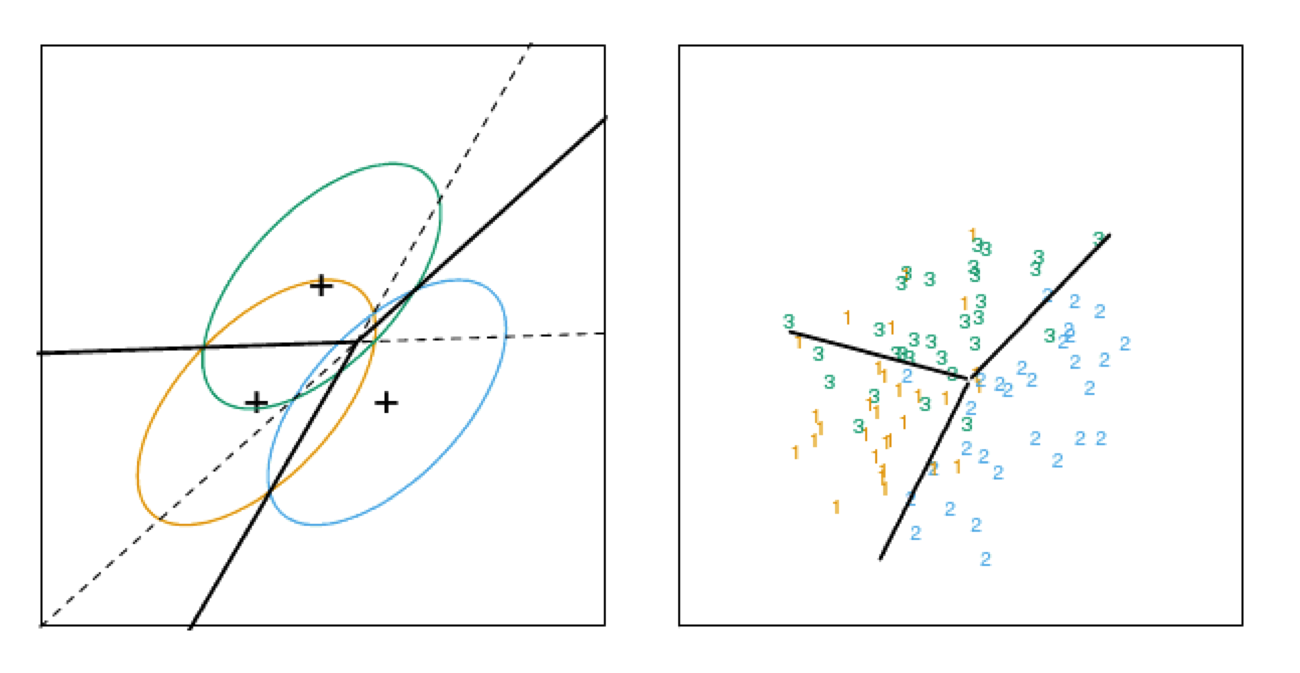
\includegraphics[width=1.0\textwidth]{fig4_5.png}
\caption{\label{fig:lda3class}Decision boundaries between 3 classes modeled using bivariate normals with equal covariance.[HTF Fig.\ 4.5]}
\end{figure}

\subsection{Linear Discriminant Function}
Formally speaking, the \emph{linear discriminant functions} have the form
$$
\delta_k(x) = x^\top \Sigma^{-1} \mu_{k} - \frac{1}{2} \mu_{k}^{\top} \Sigma^{-1} \mu_{k} + \log \pi_{k}
$$
with decision rule:
$$
G(x) = \underset{k}{\arg\max} \, \delta_{k}(x)
$$

Assuming we've already calculated the mean and covariance and we've estimated the prior, to use this as a classifier we take an observation $x$, plug this into discriminant function for each class and see which one yields the maximum discriminant function value.

If the covariance matrices are spherical (i.e., $\Sigma\propto I$) and the priors are equal (e.g., sandpipers just as likely as hawks at a campsite), the decision boundary is simply the perpendicular bisector of the line joining the two means.  Changing the prior (or class balance) has the effect of shifting the decision boundary along that line.  In the case of non-spherical covariance matrices, as in Fig.\ \ref{fig:lda3class}, the decision boundary still bisects the line joining the means but is no longer perpendicular.

\subsection{Parameter Estimation}

We've been assuming that the priors, mean and covariance were estimated for us thus far.  Here's how you estimate them.

Priors:
$$
\hat{\pi}_{k} = \frac{N_k}{N}
$$
where $N_k$ is the number of class $k$ observations and $N$ is the total number of observations.

Sample mean:
$$
\hat{\mu}_{k} = \frac{1}{N_k} \sum_{g_i = k} x_i
$$
Here the sum is over the feature vectors belonging to class $k$.

Sample covariance:
$$
\hat{\Sigma} = \frac{1}{N-K} \sum_{k=1}^{K} \sum_{g_i = k} (x_i-\hat{\mu}_k)(x_i - \hat{\mu}_k)^\top
$$

Covariance matrices are also known as \emph{centered second moment} matrices.  The centering operation refers to subtracting the class mean.  The second moments refer to the sum of the outer products of the feature vectors with themselves.  You can think of this as the vector counterpart to squaring for scalars.  Each term in that sum is a $p\times p$ matrix containing all the possible products between pairs of entries in a feature vector.  The outer summation is over all $K$ classes; we can do this \emph{pooling} operation because we assumed that all classes have same covariance matrix.  


\subsection{Comparison with Logistic Regression}

The log posterior odds in LDA has the form 
$$
\alpha_{k0} + \alpha_{k}^{\top}x
$$
which looks an awful lot like
$$
\beta_{k0} + \beta_{k}^{\top}x
$$
from logistic regression.  The difference lies in how the coefficients are estimated. The bottom line is that the results of using LDA and LR are often very similar.  LR is a discriminative classifier. LR has the advantage of making fewer assumptions about how the data are distributed.  LDA is a generative classifier. LDA has the advantage of offering low dimensional projections of the data, useful for visualization.  LDA assumes multivariate Gaussian distribution, so it can generate additional data as needed. 

We'll discuss this in the next lecture.


\end{document}
